\section{Method}
\label{sec:method}

\paragraph{Notation.}
S0 is cross-entropy pre-training of the ImageNet-initialised network on the base classes, R the recovery epochs of the same loss after pruning, M episodic (prototypical) meta-training, G the same episodes with the learning rate set to zero (a gradient probe), and P a pruning step. A \emph{mid channel} is an output channel of the first convolution of a residual block, the inner channel that we remove. All methods of one class partition start from the same S0 network.

\paragraph{Episodes and classifier.}
An episode draws $N{=}5$ classes, $K$ labelled support images and $Q{=}15$ query images per class. We embed an image with the 512-d global-average-pooled output of a ResNet-18, L2-normalise it, average the support embeddings of each class into a prototype, and give each query the label of the most similar prototype under cosine similarity. Base classes are the only classes the network sees, whether for training, for pruning decisions or for the calibration statistics below. Novel classes appear at evaluation and nowhere else.

\paragraph{What is pruned.}
A ResNet-18 has eight basic blocks, each with two $3{\times}3$ convolutions. We remove output channels of the first convolution, together with their BatchNorm entries and the matching input slices of the second ($1920$ ``mid'' channels in total). The stem, the shortcuts and the block outputs keep their width, so no index has to be matched across a residual addition; He et al.~\cite{he2017channel} prune residual branches the same way. The budget is the share of the $11.18$\,M trunk parameters that remain, counted on the pruned network (the classifier is a parameter-free prototype head and is not counted). To spread a budget over depth, every score in this paper uses one rule: block $b\in\{0,\dots,7\}$ keeps a fraction $\kappa\,(1-\tau\,b/7)$ of its mid channels, with $\tau{=}0.5$ and $\kappa$ found by bisection. Deep blocks hold most of the weights, so they lose most of the channels. Since the rule is shared, two scores differ only in which channels they keep inside a block.

\paragraph{Scores.}
All scores are computed on a calibration set of $40$ images per base class, without augmentation. Four are standard: random; the $\ell_1$ norm of the filter~\cite{li2017pruning}; the BatchNorm scale $|\gamma|$~\cite{liu2017slimming}; and a first-order Taylor term~\cite{molchanov2017pruning}, the mean over images of $\lvert\sum_{x,y} a\,\partial L/\partial a\rvert$ for the post-ReLU mid activation $a$. The loss $L$ is the cross-entropy of a cosine nearest-prototype classifier whose prototypes are the calibration class means under the current network, so no trained head has to survive the earlier stages.

DACIS combines three per-channel quantities. $\Gs_c$ is the mean $\ell_2$ norm of $\partial L/\partial W_c$ over calibration batches of $64$ images, where $W_c$ is the filter of channel $c$. $\Vs_c$ is the variance, across calibration images, of the spatially pooled activation of the channel. $\Ds_c$ is the Fisher ratio of that pooled activation over the class labels, $\Ds_c=\sum_k n_k(\mu_{kc}-\mu_c)^2\big/\sum_k\sum_{i\in k}(a_{ic}-\mu_{kc})^2$, the between-class over within-class scatter used in linear discriminant analysis~\cite{fisher1936}. Each quantity is replaced by its rank inside the block, scaled to $[0,1]$ (written $\mathrm{rk}$), and the score is
\begin{equation}
  \mathrm{DACIS}_c=\lambda_G\,\mathrm{rk}(\Gs_c)+\lambda_V\,\mathrm{rk}(\Vs_c)+\lambda_D\,\mathrm{rk}(\Ds_c),
  \label{eq:dacis}
\end{equation}
with weights $(\lambda_G,\lambda_V,\lambda_D)=(0.3,0.2,0.5)$ that we fixed before running any experiment reported here. They were not tuned on the novel classes; Sec.~\ref{sec:lambda} examines them on held-out validation classes. Ranks rather than raw values keep the heavy tails of $\Ds$ and $\Gs$ from deciding the sum.

\begin{figure*}[t]
  \centering
  % Figure 1: how a scene is classified by the pruned network (top) and the PMP schedule (bottom). TikZ; no data in this figure.
\begin{tikzpicture}[
    font=\footnotesize,
    box/.style={draw, rounded corners=1.5pt, minimum height=0.7cm, align=center, inner sep=2.5pt, line width=0.5pt},
    prune/.style={box, fill=red!10, draw=red!60!black},
    train/.style={box, fill=blue!8, draw=blue!50!black},
    base/.style={box, fill=gray!12, draw=gray!70!black},
    keep/.style={box, fill=green!12, draw=green!45!black},
    arr/.style={-{Stealth[length=4.5pt]}, line width=0.6pt},
    bar/.style={draw=blue!60!black, fill=blue!35, line width=0.3pt},
    cut/.style={draw=red!70!black, fill=white, dash pattern=on 1pt off 0.8pt, line width=0.35pt}
]
  % ---- (a) one scene through the pruned network -------------------------------------------------------
  \node[anchor=west, font=\footnotesize\bfseries] at (-0.7,1.25) {(a) An image becomes a label};
  \node[inner sep=0pt, draw, line width=0.4pt] at (-0.58,0) {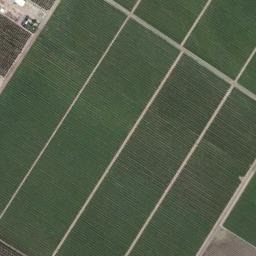
\includegraphics[width=1.05cm,height=1.05cm]{img_aerial.jpg}};
  \node[inner sep=0pt, draw, line width=0.4pt] at (0.58,0) {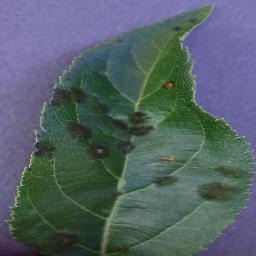
\includegraphics[width=1.05cm,height=1.05cm]{img_leaf.jpg}};
  \node[align=center, font=\scriptsize] at (0,-1.15) {input images: aerial\\scene, leaf photo\\(13-band patches too)};
  \foreach \cx/\pat in {2.3/{0/1,1/1,2/1,3/0,4/1,5/1}, 3.6/{0/1,1/0,2/1,3/1,4/0,5/1}, 4.9/{0/0,1/1,2/0,3/1,4/0,5/1}, 6.2/{0/0,1/0,2/1,3/0,4/0,5/1}} {
    \draw[rounded corners=1.5pt, fill=white, line width=0.5pt] (\cx-0.5,-0.62) rectangle (\cx+0.5,0.62);
    \foreach \j/\k in \pat {
      \ifnum\k=1 \draw[bar] ({\cx-0.38+0.15*\j},-0.4) rectangle ++(0.08,0.8);
      \else \draw[cut] ({\cx-0.38+0.15*\j},-0.4) rectangle ++(0.08,0.8); \fi
    }
  }
  \foreach \x in {2.8,4.1,5.4} \draw[arr] (\x,0) -- ++(0.3,0);
  \draw[arr] (1.2,0) -- (1.77,0);
  \node[text width=5.8cm, align=center, font=\scriptsize] at (4.25,-1.3) {ImageNet-pretrained trunk (ResNet-18 or MobileNetV2): the inner channels of each block are scored and the lowest scorers (dashed) are removed; deeper blocks lose more};
  \node[train, minimum width=1.9cm] (pool) at (8.55,0) {global average\\pool, L2 norm};
  \draw[arr] (6.7,0) -- (pool.west);
  \foreach \i/\v in {0/15,1/60,2/30,3/80,4/20,5/55,6/40,7/70} \fill[blue!\v] ({10.0+0.15*\i},-0.17) rectangle ++(0.13,0.34);
  \node[font=\scriptsize] at (10.55,0.42) {embedding};
  \draw[arr] (pool.east) -- (9.93,0);
  \node[keep, minimum width=2.1cm] (cos) at (12.45,0) {cosine similarity\\to 5 prototypes};
  \draw[arr] (11.25,0) -- (cos.west);
  \node[base, minimum width=1.3cm] (out) at (14.75,0) {label =\\nearest};
  \draw[arr] (cos.east) -- (out.west);
  \node[base, minimum width=2.9cm] (sup) at (12.45,-1.55) {$K$ support scenes per class:\\mean embedding = prototype};
  \draw[arr] (sup.north) -- (cos.south);
  % ---- (b) the PMP schedule -----------------------------------------------------------------------------
  \node[anchor=west, font=\footnotesize\bfseries] at (-0.7,-2.55) {(b) The PMP schedule};
  \node[base] (s0) at (0.45,-3.45) {ImageNet\\weights};
  \node[train, right=0.28cm of s0] (ce) {S0: CE on\\base classes};
  \node[prune, right=0.28cm of ce] (p1) {P1: prune\\to 60\%};
  \node[train, right=0.28cm of p1] (r1) {R: recover\\with CE};
  \node[train, right=0.28cm of r1] (m) {M: 1000\\episodes};
  \node[prune, right=0.28cm of m] (p2) {P2: prune\\to budget};
  \node[train, right=0.28cm of p2] (r2) {R: recover\\with CE};
  \foreach \a/\b in {s0/ce, ce/p1, p1/r1, r1/m, m/p2, p2/r2} \draw[arr] (\a) -- (\b);
  \node[box, dashed, draw=red!60!black, below=0.5cm of p2, font=\scriptsize] (g) {$G_{\mathrm{meta}}$: filter-gradient\\norm collected in M};
  \draw[arr, dashed, red!60!black] (m.south) |- (g.west);
  \draw[arr, dashed, red!60!black] (g.north) -- (p2.south);
  \node[right=0.4cm of r2, align=left, font=\scriptsize] {\textcolor{blue!50!black}{$\blacksquare$} training\\\textcolor{red!60!black}{$\blacksquare$} pruning};
\end{tikzpicture}

  \caption{The PMP schedule and the DACIS score. Blue boxes are training stages (S0 and R use cross-entropy on the base classes, M is episodic), red boxes are pruning steps. P1 prunes to $60\%$ of the parameters, M accumulates the mean filter-gradient norm $G_{\mathrm{meta}}$ of the episode loss, and P2 prunes to the target budget with a score that also uses $G_{\mathrm{meta}}$.}
  \label{fig:overview}
\end{figure*}

\paragraph{The PMP schedule.}
We write S0 for supervised cross-entropy training of the ImageNet-initialised network on the base classes, R for the recovery epochs of the same loss (one on PlantVillage, two on the Earth-observation sets), M for episodic training, and P for a pruning step. Figure~\ref{fig:overview} shows the full schedule. After S0, P1 prunes to $60\%$ of the parameters, R recovers, and M runs $1000$ episodes ($5$-way, $5$-shot, $15$ queries) of prototypical training with frozen BatchNorm statistics, in the manner of Meta-Baseline~\cite{chen2021metabaseline}. While M runs we accumulate, for every mid channel, the mean norm of the episode-loss gradient with respect to its filter, $G_{\mathrm{meta}}$. P2 prunes to the target budget with
$\mathrm{DACIS}_c\,\bigl(1+\gamma\,\mathrm{rk}(G_{\mathrm{meta},c})\bigr)$, $\gamma{=}1$, recomputed on the meta-trained network, and a last R repairs the damage. Table~
ef{tab:schedules} lists the seven schedules we compare. The alternatives are P (prune once, then R), P$\to$M, M$\to$P and P$\to$M$\to$P$\to$M. Two controls separate what a stage contributes. P$\to$M with twice the episodes tests whether extra stages help only because they train longer. P$\to$G$\to$P replaces M by $200$ episodes with the learning rate set to zero, so the network is untouched and only the gradient statistic $G_{\mathrm{meta}}$ is collected; it asks whether the information in the meta stage is useful without its weight updates. The learning rate of M was chosen on validation classes (Sec.~\ref{sec:results}).

\begin{table}[t]
  \centering\footnotesize\setlength{\tabcolsep}{4pt}
  \begin{tabular}{@{}ll@{}}
    \toprule
    Schedule & Steps after S0 \\
    \midrule
    P & P(30\%), R \\
    P$\to$M & P(30\%), R, M \\
    M$\to$P & M, P(30\%), R \\
    P$\to$G$\to$P & P(60\%), R, G, P(30\%), R \\
    PMP & P(60\%), R, M, P(30\%), R \\
    PMPM & PMP, then M \\
    P$\to$M, $2\times$ & P(30\%), R, M with twice the episodes \\
    \bottomrule
  \end{tabular}
  \caption{The seven schedules. P(x) prunes to the share x of the parameters; G collects the gradient statistic without updating a weight.}
  \label{tab:schedules}
\end{table}
